\section*{Problem 3}

\begin{figure}[H]
\caption*{}
\centering
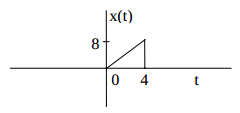
\includegraphics[width=0.4\textwidth]{figs/c2p3.png}
\label{fig:c2p3}
\end{figure} 

\subsection*{Solution}

Taking the derivative of $x(t)$ we get:

\begin{figure}[H]
\caption{Derivative $\dot{x}$}
\centering
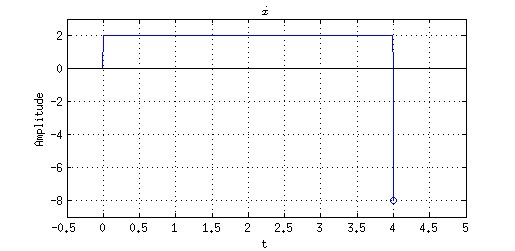
\includegraphics[width=0.6\textwidth]{figs/c2p3dotx.png}
\label{fig:c2p3dotx}
\end{figure}


Lets call $x_{p1}(t)$ and $X_{p1}(\omega)$ the function in time domain of the first point 
and its Fourier Transform respecively. 
We can express the first derivative of our function in terms of such function as:

\begin{equation*}
\dot{x}(t) = x_{p1}(t/2) - 8 \delta(t-4)
\end{equation*} 

As we can see from (\ref{eq:c22e}) the scale in time is reflected inversely
in the frecuency domain. 

\begin{equation*}
\begin{aligned}
j \omega X(\omega) &= X_{p1}(2 \omega) - 8 e^{-4 j \omega} \\
 &= 4 Sa(2 \omega) e^{- 2 j \omega}- 8e^{-4 j \omega} \\
X(\omega) &= \frac{4 j}{\omega} e^{-2 j \omega} [2 e^{-2 j \omega}- Sa(2 \omega)]
\end{aligned}
\end{equation*} 

The plot of the magintude and angle of $X(\omega)$ is:
\zcodemat{sources/c2p3a.m}{Plot of Magnitude and Angle}

\begin{figure}[H]
\caption{Magnitude $|X(\omega)|$ and Angle}
\centering
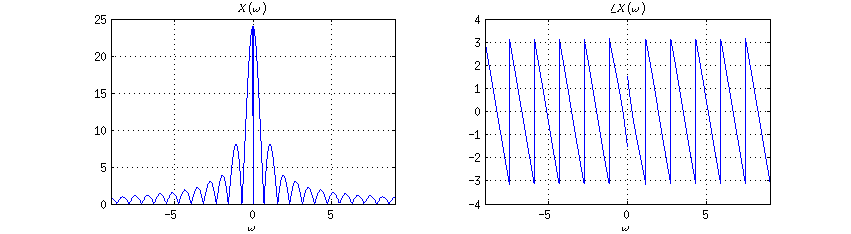
\includegraphics[width=1.0\textwidth]{figs/c2p3a.png}
\label{fig:c2p3a}
\end{figure} 

